% !TeX Options = -shell-escape

\documentclass[10pt]{beamer}

\usetheme[progressbar=frametitle, block=fill]{metropolis}
\usepackage{xcolor}
\usepackage{multirow}
\usepackage{pgfpages}
\usepackage{pifont}
\usepackage[utf8]{inputenc}
\usepackage[T1]{fontenc}
\usepackage{tikz}
\usetikzlibrary{arrows,shapes}
\usepackage{csquotes}
\usepackage{textpos}
\usepackage[english]{babel}
\newcommand{\cmark}{\ding{51}}
\newcommand{\xmark}{\ding{55}}
\setbeamertemplate{note page}{\insertnote}
%\setbeameroption{show notes on second screen=left}

\setbeameroption{hide notes}
\definecolor{amethyst}{rgb}{0.5, 0.4, 1.0}
\definecolor{amethystgrey}{rgb}{0.85, 0.85, 1.0}
\definecolor{amethystdark}{rgb}{0.4, 0.3, 0.9}
\definecolor{orangedark}{rgb}{0.0, 0.9, 0}
\definecolor{titlebg}{HTML}{fbf8ff}
\definecolor{font}{HTML}{23373b}
\setbeamercolor{frametitle}{fg= font, bg=titlebg}
\setbeamercolor{progress bar}{ fg = amethyst, bg= amethystgrey }
\setbeamercolor{alerted text}{fg=amethystdark}

\addtobeamertemplate{frametitle}{}{%
\begin{textblock*}{100mm}(1\textwidth, -1cm)

\includegraphics[height=0.97cm]{graphics/TT_Logo_bckg.png}
\end{textblock*}}


\usepackage{booktabs}
\usepackage[scale=2]{ccicons}

\usepackage{minted}

\usepackage{pgfplots}

\usepackage{xspace}

\title{C++20 Coroutines}
\subtitle{What's next?}
\date{}
\author{Dawid Pilarski}
\institute{dawid.pilarski@panicsoftware.com \\ \href{http://blog.panicsoftware.com}{blog.panicsoftware.com} \\ dawid.pilarski@tomtom.com}

\begin{document}

\maketitle

\section{Introduction}
\begin{frame}{Agenda}
	\tableofcontents
\end{frame}

\begin{frame}{Questions...}

\vfill
\centerline{Time is rather tight.}
\centerline{Please hold your questions till the end.}
\vfill

\end{frame}

\begin{frame}{Who am I?}
			\centering \alert{Dawid Pilarski}
			\vskip 1em
	\begin{columns}[onlytextwidth]
		\begin{column}{0.7\textwidth}
			\begin{itemize}
				\item Senior Software Developer in TomTom
				\item Member of the ISO/JTC1/SC22/WG21
				\item Member of the PKN KT {\tiny(programming languages)}
				\item C++ blog writer
			\end{itemize}
		\end{column}
		\begin{column}{0.29\textwidth}
				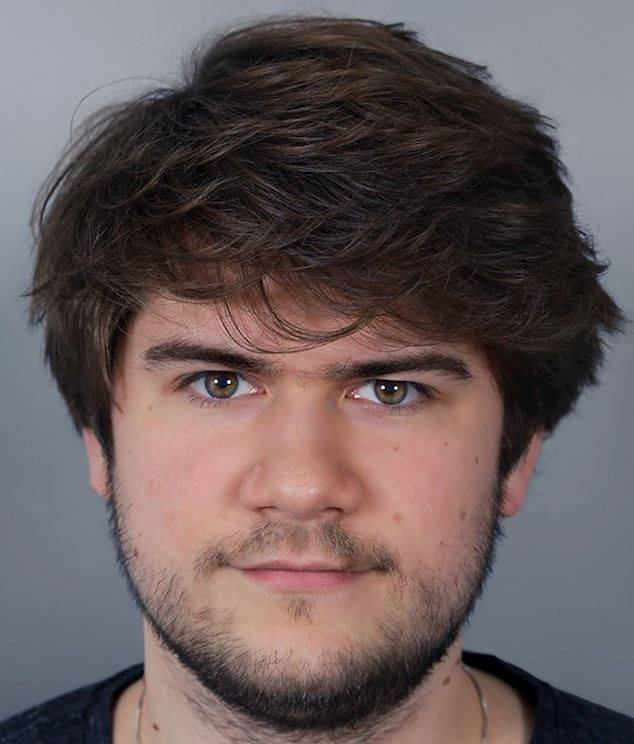
\includegraphics[width=\linewidth]{Dawid_Pilarski.jpg}				
		\end{column}	
	\end{columns}
\end{frame}

\section{Quick refresh about the coroutines.}

\begin{frame}{What are the coroutines?}
\vfill

\begin{description}
	\item [Subroutine] Is a sequence of program instructions that performs a specific task, packaged as a unit.
	\item [Function] Is a subroutine
	\item [Coroutine] Is generalization of the function.
\end{description}

\vfill
\end{frame}

\begin{frame}{What are the coroutines?}
	\alert{\only{Function}<1>\only{Coroutine}<2->} can be:
	\begin{itemize}
		\item called
		\item returned from
		\item<2-|alert@2> \alert<+>{suspended}
		\item<3-|alert@3> resumed from
		\item<4-|alert@4> created
		\item<5-|alert@5> destroyed
	\end{itemize}
\end{frame}

\begin{frame}{Coroutine flowchart}

\begin{columns}
\begin{column}{0.48\linewidth}
  \centering
  Function's flow:
  \vskip 2em
  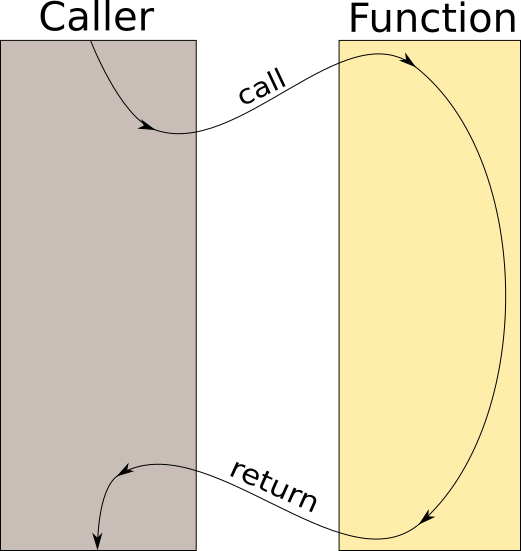
\includegraphics[width=0.8\linewidth]{graphics/function-call.png}
\end{column}
\begin{column}{0.48\linewidth}
  \centering
  Coroutine flow:
  \vskip 2em
  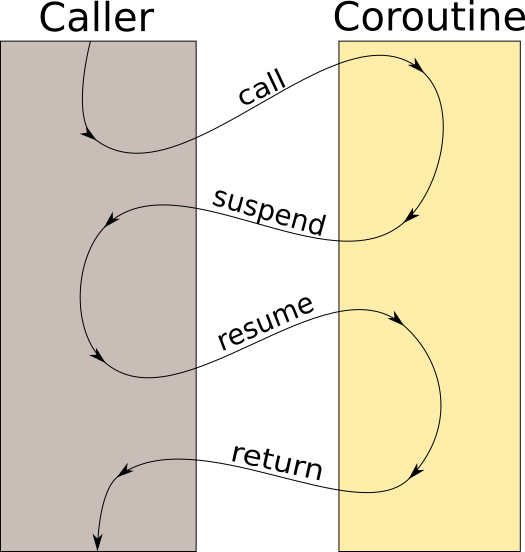
\includegraphics[width=0.8\linewidth]{graphics/coroutine-workflow.png}
\end{column}

\end{columns}

\end{frame}

\begin{frame}{How to implement custom coroutine types.}
	Creating custom coroutine type is not easy:
	\begin{itemize}[<+->]
		\item C++ provides keywords \alert{only}.
		\item \alert{Developer must implement} what keywords do.
	\end{itemize}

	\vfill

	\only{This means:}<3->
	\begin{itemize}[<+->]
		\item Implementation of promise\_type ({\fontfamily{ptm}\selectfont\texttildelow}6 functions)
		\item Implementation of the co\_await  keyword ({\fontfamily{ptm}\selectfont\texttildelow}3 functions)
	\end{itemize}

	\vfill

	\only{You need to remember to implement on average \alert{9 functions}.}<5>
\end{frame}

\begin{frame}{Coroutine declaration}
  \vfill
  \begin{center}
  \begin{minipage}{0.8\linewidth}
  \inputminted{c++}{code-examples/intro/declaration.hpp}
  \end{minipage}
  \end{center}
  \vfill

  \begin{itemize}[<+->]
  	\item Whether the function is a coroutine depends on \alert{it's definition}.
  	\item If function is a coroutine it's \alert{return type must support coroutines}.
  \end{itemize}
  
\end{frame}

\begin{frame}{Promise\_type}
	Type supports coroutines \alert{if it has promise\_type}.
	\vfill

	promise\_type can be:
	\begin{itemize}
		\item member of the class
		\item member of the specialization of the coroutine\_traits<returned\_type>
	\end{itemize}
\end{frame}

\begin{frame}{Promise\_type}
	\centerline{Promise\_type controls coroutine's behavior.}
	\vfill

	\begin{columns}
		\begin{column}{0.48\linewidth}
			\begin{footnotesize}
			\begin{itemize}[<+-|alert@+>]
				\item \texttt{awaitable initial\_suspend();}
				\item \texttt{awaitable final\_suspend();}
				\item \texttt{return\_type get\_return\_object();}
				\item \texttt{void unhandled\_exception();}
			\end{itemize}
			\end{footnotesize}	
		\end{column}
		\begin{column}{0.48\linewidth}
			\begin{footnotesize}
			\begin{itemize}
				\item<1- |alert@1> \texttt{suspension at the beginning}
				\item<2- |alert@2> \texttt{suspension at the end}
				\item<3- |alert@3> \texttt{how to create \\ return\_type}
				\item<4- |alert@4> \texttt{handling unhandled exception}
			\end{itemize}
			\end{footnotesize}	
		\end{column}
	\end{columns}
\end{frame}

\begin{frame}{Keywords and promise\_type}
	Promise\_type is also responsible for keyword's actions:
	\vfill

	\begin{columns}
		\begin{column}{0.48\linewidth}
			\begin{footnotesize}
			\begin{itemize}[<+-|alert@+>]
				\item \texttt{co\_return V;}
				\item \texttt{co\_return;}
				\item \texttt{co\_yield V;}
			\end{itemize}
			\end{footnotesize}	
		\end{column}
		\begin{column}{0.48\linewidth}
			\begin{footnotesize}
			\begin{itemize}[<+-|alert@+>]
				\item<1- |alert@1> \texttt{p.return\_value(V);}
				\item<2- |alert@2> \texttt{p.return\_void();}
				\item<3- |alert@3> \texttt{co\_await p.yield\_value();}
			\end{itemize}
			\end{footnotesize}	
		\end{column}
	\end{columns}
\end{frame}

\begin{frame}{co\_await}
	In order to support \alert{co\_await} expressions, the argument (awaitable) must:
	\begin{itemize}[<+-|alert@+>]
		\item have \texttt{awaiter operator co\_await} defined, or
		\item have global \texttt{awaiter operator co\_await(A)} support, or
		\item implement 3 functions:
		\begin{itemize}
			\item \texttt{bool await\_ready()}
			\item \texttt{await\_suspend(coroutine\_handle<P>)} returning
			\begin{itemize}
				\item void 
				\item bool
				\item another \texttt{coroutine\_handle}
			\end{itemize}
			\item \texttt{T await\_resume()}
		\end{itemize}
	\end{itemize}
\end{frame}

\section{Missing coroutines parts}

\begin{frame}{Type erasure}
	

\end{frame}

\begin{frame}{asynchronous RAII}

\end{frame}


\section{RVO or the co\_await}

\begin{frame}{What is RVO?}
\centerline{\alert{RVO} - Return Value Optimization.}

\vfill

Allows to avoid unnecessary copy or move construction of the values returned from the function. \\
\pause
For example:


\inputminted[frame=single]{c++}{code-examples/RVO_examples/example.cpp}



\end{frame}

\begin{frame}[fragile]{RVO on regular functions}

\begin{columns}[T]
\begin{column}{0.4\linewidth}
\centerline{regular function}
\vfill
\inputminted{c++}{code-examples/RVO_examples/regular_function_rvo.cpp}
\vfill
\end{column}
\begin{column}{0.55\linewidth}
\centerline{transformed by compiler into:}
\vfill
\inputminted{c++}{code-examples/RVO_examples/transformed_function_rvo.cpp}
\vfill
\end{column}
\end{columns}

\end{frame}

\begin{frame}{Why RVO is not possible with co\_await}
\begin{columns}[T]
\begin{column}{0.3\linewidth}
\centerline{expression}
\vfill
\inputminted{c++}{code-examples/RVO_examples/co_await.cpp}
\vfill

\begin{enumerate}
	\item<2-> On \alert{await\_suspend} coroutine gets executed
	\item<3-> On \alert{await\_resume} result is returned
\end{enumerate}

\end{column}
\begin{column}{0.55\linewidth}
\centerline{transformed by compiler into:}
\vfill
\begin{onlyenv}<2->
\inputminted[highlightlines={5,8}]{c++}{code-examples/RVO_examples/transformed_co_await.cpp}
\tikz[baseline,remember picture]{\node[anchor=base] at (6, 1.3) (t1){};
\tikz[remember picture] \node[coordinate] at (6,2.5) (n1) {};
}
\begin{tikzpicture}[remember picture,overlay] 
        \path[->]<1-> (n1) edge [draw=magenta, thick, bend left] (t1);
\end{tikzpicture}
\end{onlyenv}
\only{\inputminted{c++}{code-examples/RVO_examples/transformed_co_await.cpp}}<1>
\vfill
\end{column}
\end{columns}
\end{frame}

\begin{frame}{How to resolve the issue [P1663R0]}

\begin{columns}[T]
\begin{column}{0.3\linewidth}

\begin{enumerate}[<+-| alert@+>]
	\item Remove \alert{await\_resume} function.
	\item \alert{await\_suspend} will will create return result
	\item Remove \alert{await\_ready} function.
\end{enumerate}
\end{column}

\begin{column}{0.6\linewidth}
\begin{onlyenv}<1-2>
\inputminted{c++}{code-examples/RVO_examples/transformed_co_await.cpp}
\begin{tikzpicture}[remember picture, overlay]
\draw[draw=red] (0.25,1.20) -- (4.5,1.20);
\end{tikzpicture}
\end{onlyenv}

\begin{onlyenv}<2>
\begin{tikzpicture}[remember picture, overlay]
\draw [draw=blue!20, fill=blue!90, opacity=0.1] (0.7, 3.0) rectangle (5.2, 3.35);
\end{tikzpicture}
\end{onlyenv}

\begin{onlyenv}<3>
\inputminted{c++}{code-examples/RVO_examples/transformed_co_await_no_ready.cpp}

\begin{tikzpicture}[remember picture, overlay]
\draw[draw=red] (0.25,3.15) -- (5.5,3.15);
\draw[draw=red] (0.25,1.75) -- (5.5,1.75);
\draw [draw=blue!20, fill=blue!90, opacity=0.1] (0.7, 2.05) rectangle (5.2, 2.40);
\end{tikzpicture}
\end{onlyenv}

\begin{onlyenv}<4>
\inputminted{c++}{code-examples/RVO_examples/transformed_co_await_simplified.cpp}
\end{onlyenv}
\end{column}

\end{columns}

\end{frame}

\begin{frame}{Extensions to the coroutine\_handle}
	Two additional functions in the coroutine\_handle are needed.

	\begin{itemize}[<+-| alert@+>]
		\item set\_value(T)
		\item set\_value\_from(Arg...)
		\item set\_exception(exception\_ptr)
	\end{itemize}
	
	\onslide<+->{On coroutine resumption the compiler will generate code to check whether the exception was saved with \alert{set\_exception} and will rethrow it when needed.}


\end{frame}

\begin{frame}{Example of the yield\_value}
\only{
\inputminted[highlightlines={1}]{c++}{code-examples/RVO_examples/yield_value.cpp}
}<1>

\only{
\inputminted[highlightlines={4-7}]{c++}{code-examples/RVO_examples/yield_value.cpp}
}<2>

\only{
\inputminted[highlightlines={6}]{c++}{code-examples/RVO_examples/yield_value.cpp}
}<3>

\only{
\inputminted[highlightlines={9-14}]{c++}{code-examples/RVO_examples/yield_value.cpp}
}<4>

\only{
\inputminted[highlightlines={11-12}]{c++}{code-examples/RVO_examples/yield_value.cpp}
}<5>

\only{
\inputminted[highlightlines={13}]{c++}{code-examples/RVO_examples/yield_value.cpp}
}<6>

\end{frame}

\begin{frame}{How do compiler know the result of the co\_await?}
	With removal of the \alert{await\_ready} the compiler no longer knows about the co\_await returned type.
	\vfill

	We will need to guide the compiler. The proposal 
	P1663R0 proposes to add member \alert{await\_result\_type} to the Awaiter.
	\vfill

\end{frame}

\begin{frame}{RVO summary}
\begin{columns}[T]

\begin{column}{0.48\linewidth}
\centerline{pros}
\begin{itemize}[<+-| alert@+>]
	\item very simplified awaiter concept
	\item savings in CPU cycles
	\begin{itemize}
		\item Avoiding unnecessary move construction
	\end{itemize}
	\item savings in memory
	\begin{itemize}
		\item no temporary variable created
		\item allocated coroutine state is smaller
	\end{itemize}
\end{itemize}
\end{column}
\begin{column}{0.48\linewidth}
\centerline{cons}
\begin{itemize}[<+-| alert@+>]
	\item removing \alert{await\_ready} makes \alert{co\_await} always suspend the coroutine (even if not needed)
	\item a need to support RVO manually (with the help of \alert{construct\_in\_place})
	\item proposed RVO does not consider synchronous coroutines - only \alert{co\_await} keyword.
\end{itemize}
\end{column}
\end{columns}

\end{frame}

\begin{frame}{return value [and|or] return void}

\end{frame}

\section*{Thank you for your attention!}

\begin{frame}{Special thank you! goes to:}
	\begin{itemize}
		\item Gor Nishanov
		\item Lewiss Baker	
	\end{itemize}

	for making coroutines 
\end{frame}

\begin{frame}{Bibliography and further reading}
\begin{columns}
\begin{column}{0.48\linewidth}
	\begin{itemize}
		\item Lewiss Baker's Assymetric transfer blog
		\item newest C++ draft
		\item My blog - blog.panicsoftware.com
	\end{itemize}
\end{column}
\begin{column}{0.48\linewidth}
	\begin{itemize}
		\item James McNellis - "Introduction to the C++ Coroutines"
		\item Gor Nishanov - any video about the coroutines
		\item Toby Allsopp - "Coroutines: what can't they do?"
	\end{itemize}
\end{column}

\end{columns}
\end{frame}

\begin{frame}{Questions?}
\vfill
\centering Questions?
\vfill
\end{frame}

\end{document}